\documentclass[a4paper, 12pt]{article}
\usepackage{azzam-light}

\begin{document}
\title{Geometri Dua Dimensi}
\maketitle
\begin{enumerate}
\section{Angle Chasing}
    \item Jika $I$ adalah titik pusat lingkaran dalam atau titik bagi (incenter) dari $\triangle ABC$ maka buktikan bahwa
        $\angle BIC = 90^\circ + \frac{1}{2}A.$

    \item Misalkan $ABCDE$ adalah sebuah segilima konveks sedemikian sehingga $BCDE$ adalah persegi dengan pusat $O$ dan $\angle A = 90^\circ$. Buktikan bahwa $\overline{AO}$ membagi dua sama besar $\angle BAE$.

    \item Misalkan $O$ dan $H$ masing-masing menyatakan titik pusat lingkaran luar dan titik tinggi dari sebuah segitiga lancip $\triangle ABC$. Tunjukkan bahwa $\angle BAH = \angle CAO$.

    \item (OSN SMP 2003) Perhatikan gambar susunan tiga persegi di bawah. 
    
    Buktikan bahwa $\angle BAX+\angle CAX=45^{\circ}$.
    
        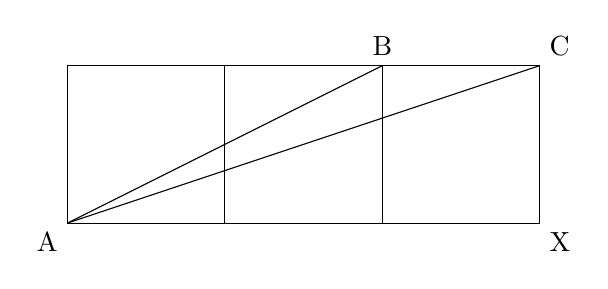
\begin{tikzpicture}[scale=1]
        % Define the unit width of each square
        \def\unitw{2} 
        
        % Draw the main rectangle (3 squares wide, 1 square high)
        \draw (0,0) rectangle (3*\unitw, \unitw);
        
        % Draw vertical lines for the squares
        \draw (\unitw,0) -- (\unitw,\unitw);
        \draw (2*\unitw,0) -- (2*\unitw,\unitw);
        
        % Draw the diagonal lines from A
        \draw (0,0) -- (2*\unitw, \unitw); % Line to B's position
        \draw (0,0) -- (3*\unitw, \unitw); % Line to C's position
        
        % Place the labels
        \node[below left] at (0,0) {A};
        \node[above] at (2*\unitw, \unitw) {B};
        \node[above right] at (3*\unitw, \unitw) {C};
        \node[below right] at (3*\unitw, 0) {X};
    \end{tikzpicture}

    \item (OSN SMP 2013) Diketahui ABC adalah segitiga lancip dengan titik - titik sudutnya terletak pada lingkaran yang berpusat di titik O. Titik P terletak pada sisi BC sehingga AP adalah garis tinggi segitiga ABC. Jika $\angle ABC+30^{\circ} \le \angle ACB$, buktikan bahwa $\angle COP+\angle CAB < 90^{\circ}$.
        
\section{Length Chasing}
    \item (Teorema Pitot) Misalkan $ABCD$ adalah sebuah segiempat. Jika sebuah lingkaran dapat menyinggung keempat sisinya, buktikan bahwa $AB + CD = BC + DA$.
    \begin{figure}[H]
        \includegraphics[width=0.4\linewidth]{0Figure/pitot-theorem.png}
    \end{figure}

            \item (OSN SMA 2002)
    Diberikan segitiga $ABC$ dengan $AC > BC$. Pada lingkaran luar segitiga $ABC$ terletak titik $D$ yang merupakan titik tengah busur $AB$ yang memuat titik $C$. Misalkan $E$ adalah titik pada $AC$ sehingga $DE$ tegak lurus pada $AC$. Buktikan bahwa $AE = EC + CB$.

\section{Luas}
    \item (OSN SMP 2009) Pada suatu segitiga ABC, titik D terletak pada sisi AB dan titik E terletak pada sisi AC. Tunjukkan bahwa $\frac{\text{Luas } \triangle ADE}{\text{Luas } \triangle ABC} = \frac{AD \times AE}{AB \times AC}$.

    \item (OSN SMP 2022) Diketahui ABCD jajargenjang. Sebuah lingkaran dengan pusatnya pada perpotongan diagonal AC dan BD menyinggung AB dan CD. Lingkaran tersebut digeser sehingga menyentuh BC. Lingkaran hasil memotong diagonal BD di titik P dan Q. Jika $BP=9$, $PQ=27$, dan $DQ=48$. Tentukan luas daerah jajargenjang yang belum pernah disentuh lingkaran.

    \item (OSN SMP 2021) Diketahui daerah segi empat ABCD dengan $AB=2$ cm, $BC=8$ cm, $CD=6$ cm, $DA=7$ cm, terbagi menjadi dua daerah segitiga oleh $\overline{AC}$ yang panjangnya 9 cm. lingkaran dalam kedua segitiga menyinggung $\overline{AC}$ di titik E dan F. Jika titik pusat masing-masing lingkaran dalam segitiga adalah M dan N, serta luas daerah segitiga EFM adalah $L \text{ cm}^{2}$, tentukan nilai maksimum dari $L^{2}$.



        \item (OSN SMP 2024) Perhatikan gambar segitiga ABC berikut.
    \begin{figure}[H]
    \centering
    \includegraphics[scale=0.5]{0Figure/osn-smp-2024-3.png}
    \end{figure}
    Panjang sisi $BC=12$ cm dan $AC=8$ cm. Titik D, E, dan F berada pada sisi AB, BC, dan AC. Jika $DE=4$ cm, $AD:AB=1:3$, serta $\angle DEB$ dan $\angle DFA$ adalah sudut siku-siku, tentukan luas daerah segitiga DEF.

    \item (OSN SMP 2023) Diberikan sebuah segienam ABCDEF dengan panjang sisi 8 cm. pada setiap sisi, dibuat setengah lingkaran seperti pada gambar. Tentukan total luas daerah yang diarsir?
    \begin{figure}[H]
    \centering
    \includegraphics[scale=0.5]{0Figure/osn-smp-2023-1.png}
    \end{figure}
    
    \item (OSN SMA 2006)
    Pada segitiga $ABC$, $M$ adalah titik tengah $BC$ dan $G$ adalah titik berat segitiga $ABC$. Sebuah garis $l$ melalui $G$ memotong ruas garis $AB$ di $P$ dan ruas garis $AC$ di $Q$, dimana $P \neq B$ dan $Q \neq C$. Jika $[XYZ]$ menyatakan luas segitiga $XYZ$, tunjukkan bahwa
    $$
    \frac{[BGM]}{[PAG]} + \frac{[CMG]}{[QGA]} = \frac{3}{2}
    $$

    \newpage
    \section{Campur}


    \item (OSN SMP 2017) Terdapat 5 titik yang berbeda, $T_{1}$, $T_{2}$, $T_{3}$, $T_{4}$ dan $T$ pada sebuah lingkaran L. Misalkan $t_{ij}$ adalah jarak titik $T$ ke garis $T_{i}T_{j}$ atau perpanjangannya. Buktikan bahwa $\dfrac{t_{ij}}{t_{jk}}=\dfrac{TT_{i}}{TT_{k}}$ dan $\dfrac{t_{12}}{t_{24}}=\dfrac{t_{13}}{t_{34}}$.
    \newline
    \begin{tikzpicture}[scale=2]
        % Define the center and radius of the circle
        \coordinate (O) at (0,0);
        \def\R{1.5}
    
        % Define the points on the circle for the polygon
        % (Angles chosen to roughly match the input image)
        \coordinate (T1) at (180:\R);
        \coordinate (T2) at (220:\R);
        \coordinate (T3) at (320:\R);
        \coordinate (T4) at (30:\R);
        \coordinate (T)  at (100:\R); % The top point T
    
        % Draw the circle
        \draw (O) circle (\R);
    
        % Draw the polygon segments
        \draw (T1) -- (T2) -- (T3) -- (T4) -- (T) -- cycle; % This forms a pentagon
    
        % Draw the perpendicular from T1 to the tangent
        \tkzDefPointBy[projection = onto T1--T2](T)
        \tkzGetPoint{P_T1_tangent}
        \draw[dashed] (T1) -- (P_T1_tangent) -- (T);
        \tkzMarkRightAngle[size=0.15](T1,P_T1_tangent,T) % Right angle mark
    
        % Draw the perpendicular from T to the side T2-T3
        \tkzDefPointBy[projection=onto T2--T3](T)\tkzGetPoint{P_T_T2T3}
        \draw[dashed] (T) -- (P_T_T2T3);
        \tkzMarkRightAngle[size=0.15](T,P_T_T2T3,T3) % Right angle mark
    
        % Place the labels for the points
        \node[below left] at (T1) {$T_1$};
        \node[below right] at (T2) {$T_2$};
        \node[below right] at (T3) {$T_3$};
        \node[above right] at (T4) {$T_4$};
        \node[above] at (T) {$T$};
    
        % Place the labels for t12 and t23
        % For t12 (from T1 to Tangent)
        \node[above left, inner sep=1pt] at ($ (T)!0.5!(P_T1_tangent) $) {$t_{12}$};
        
        % For t23 (from T to T2T3)
        \node[right, inner sep=1pt] at ($ (T)!0.5!(P_T_T2T3) $) {$t_{23}$};
        \draw (T) -- (T3);

        \node[below] at (P_T_T2T3){$T_{23}$};
        \node[below left] at (P_T1_tangent){$T_{12}$};
    \end{tikzpicture}
    


    \item (OSN SMP 2020) Misalkan AB sebagai diameter lingkaran dan P titik diluar lingkaran. Garis PQ dan PR menyinggung lingkaran di titik Q dan R. Garis PH berpotongan tegak lurus dengan garis AB di H dan PH berpotongan AR di S. Jika $\angle QPH=40^{\circ}$ dan $\angle QSA=30^{\circ}$ tentukan $\angle RPS$.

\end{enumerate}
\end{document}